\documentclass{article}

\usepackage{times}
\usepackage{amssymb, amsmath, amsthm}
\usepackage[margin=.5in]{geometry}
\usepackage{graphicx}
\usepackage[linewidth=1pt]{mdframed}

\usepackage{import}
\usepackage{xifthen}
\usepackage{pdfpages}
\usepackage{transparent}

\newcommand{\incfig}[1]{%
    \def\svgwidth{\columnwidth}
    \import{./figures/}{#1.pdf_tex}
}

\newtheorem{theorem}{Theorem}[section]
\newtheorem{lemma}{Lemma}[section]
\newtheorem*{remark}{Remark}
\theoremstyle{definition}
\newtheorem{definition}{Definition}[section]

\begin{document}

\title{Mathematical Statistics - Assignment 7}
\author{Philip Warton}
\date{\today}
\maketitle
4.56, 4.59, 4.74 (except part e), 4.88, 4.92, 4.96 (except part d), 4.126, 4.134 (except part c), 4.142, 4.190
\section*{Problem 4.56}
    Find the conditional probability that a customer arrives during the last 5 minutes
    of the 30-minute period if it is known that no one arrives during the first 10 
    minutes of the period. We write this probability as $P(Y > 25 | Y > 10) = \frac
    {P(Y > 25)}{P(Y > 10)}$.

    \[
        P(Y > 10) = \int_0^10 \frac{1}{30} dy = \frac{1}{3}
    \]
    
    \[
        P(Y > 25) = \int_{25}^{30} \frac{1}{30} dy = \frac{1}{6}
    \]

    \[
        \frac{P(Y > 25)}{P(Y > 10)} = \frac{\frac{1}{6}}{\frac{1}{3}} = \frac{1}{2}
    \]

    So the probability that a customer arrives in the last 5 minutes given that no 
    one has arrived in the first 10 minutes is $.5$.

\section*{Problem 4.59}
    If $Z$ is a standard normal random variable, find the value $z_0$ such that

    \subsection*{(a)}
        $P(Z > z_0) = .5$ Since the normal distribution is symmetric and its mean
        is 0, we say that $z_0 = 0$.

    \subsection*{(b)}
        $P(Z < z_0) = .8463$. First note that $1 - .8463 = .1537$. Then we consult
        the table in the appendix for the standard normal distribution and we say
        $z_0 = 2.16$.

    \subsection*{(c)}
        $P(-z_0 < Z < z_0) = .90$. Using the fact that $Z$ is symmetric, we say that
        it must be a probability such that $P(Z > z_0) = .05$. Looking at our table
        of normal distribution values, we say that $z_0 = 1.65$ approximately.

    \subsection*{(d)}
        $P(-z_0 < Z < z_0) = .99$. By the same logic, we want $z_0$ such that $P(Z > z_0)
        = .005$. So we can get an approximate value using our table, that is $z_0 = 2.58$.

\section*{Problem 4.74}
    Scores on an examination are assumed to be normally distributed with mean 78 and 
    variance 36.

    \subsection*{(a)}
        What is the probability that a person taking the examination scores higher than
        72?\\\\
        The first order of business will be to convert these values to a normal distribution,
        which means we take $P(Y > 72) = P(Z > \frac{72 - 78}{\sqrt{36}}) = P(Z > \frac{-6}
        {6}) = P(Z > -1)$. Using the normal distribution table we say that this probability is,
        $P(Z > -1) = 1 - P(Z > 1) = 1 - .1587 = .8413$.

    \subsection*{(b)}
        Suppose that students scoring in the top $10\%$ of this distribution are to
        recieve a A grade. What is the minimum score a student must achieve to earn an
        A grade?\\\\
        We wish to find some integer $y$ such that $P(Y > y) = .1$. So we know that $P(Z >
        z_0) = .1 \Longrightarrow z_0 = 1.28$. Then to convert this back to a minimum score,
        we must undo the relationship $Z = \frac{Y - \mu}{\sigma}$, which means we must
        multiply by $\sigma$ then add $\mu$. So $z_0 \cdot \sigma + \mu = 1.28 \cdot 6 + 
        78 = 85.68$. This means our minimum score will be $86$.

    \subsection*{(c)}
        What must be the cutoff point for passing the examination if the examiner
        wants only the top $28.1\%$ of all scores to be passing?\\\\
        To answer this we do the same thing. $P(Z > z_0) = .281 \Longrightarrow z_0
        = .58$. Then we convert this back to a test score $z_0 \cdot \sigma + \mu = 
        .58 \cdot 6 + 78 = 81.48$. This means our cutoff for passing will be 82.

    \subsection*{(d)}
        Approximately what proportion of students have scores 5 or more points above
        the score that cuts off the lowest $25\%$.\\\\
        We want to find $-z_0$ such that $P(Z > z_0) = .25 \Longrightarrow z_0 = .67$.
        Then we wish to convert $-z_0$ to a test-point score. So $-.67(6) + 78 = 73.98$.
        This means that we wish to find how many students have scores bigger than or equal
        $74 + 5$. Finally $P(Y > 79) = P(Z > \frac{1}{6}) = .4325$ (normal probability table).

    \subsection*{(f)}
        If it is known that a student's score exceeds 72, what is the probability 
        that his or her score exceeds 84?\\\\
        We konw that $P(Y > 84 | Y > 72) = P(Z > 1 | Z > -\frac{2}{3}) = \frac{P(Z > 1)}
        {P(Z > -\frac{2}{3})}$. By looking at the table we find that this is equal to 
        $\frac{.1587}{1 - .2514} = .2120$.

\section*{Problem 4.88}
The magnitude of earthquakes recorded in a region of North America can be modeled
 as having an exponential distribution with mean 2.4, as measured on the Richter 
 scale. Find the probability that an earthquake striking this region will
    
    \subsection*{(a)}
        exceed 3.0 on the Richter scale.\\\\
        To answer this we say that the probability will have a distribution of 
        $f(y) = \frac{1}{2.4}e^{-\frac{y}{2.4}}$ for non-negative $y$. Then we want to 
        find $P(Y > 3.0)$. To find this we write $P(Y > 3) = e^{-\frac{3}{2.4}} = .2865$.

    \subsection*{(b)}
        fall between 2.0 and 3.0 on the Richter scale.\\\\
        We want $P(3.0 > Y > 2.0) = P(Y > 2.0) - P(Y > 3.0) = e^{-\frac{2}{2.4}} - .2865
         = .1481$.

\section*{Problem 4.92}
    The length of time $Y$ necessary to complete a key operation in the construction
    of houses has an exponential distribution with mean 10 hours. The formula $C = 
    100 + 40Y + 3Y^2$ relates the cost $C$ of completing this operation to the square
    of the time to completion. Find the mean and variance of $C$.\\\\
    \begin{align*}
        E(C) &= E(100 + 40Y + 3Y^2)\\
        &= 100 + 40 E(Y) + 3 E(Y^2)\\
        &= 100 + 40 (10) + 3 (2(10^2)) & \text{(see proof for mean and variance of Gamma distribution)}\\
        &= 100 + 400 + 3(200)\\
        &= 1100
    \end{align*}
    And thus we have the expectation of $C, 1100$.\\\\

    To compute the variance of $C$. First we wish to compute $E(Y^k)$ generally.
    \[
        E(Y^4) = \int_0^\infty y^k \left( \frac{y^{\alpha - 1} e ^{-y / \beta}}{\beta^\alpha \Gamma ( \alpha)}\right)dy
        = \frac{1}{\beta^\alpha \Gamma(\alpha)} \int_0^\infty y^{\alpha - 1 + k} e^{-y / \beta} dy = 
        \frac{1}{\beta^\alpha \Gamma(\alpha)}[\beta^{\alpha + k}\Gamma(\alpha + k)] = 
        \frac{\beta^k \frac{(\alpha + k)!}{\alpha !} \Gamma(\alpha)}{\Gamma(\alpha)}
    \]
    When $k = 4$, this will equal $\beta^4 (\alpha + 3)(\alpha + 2)(\alpha + 1)(\alpha)$. So since we have $Y$ is exponential,
    we say that $\alpha = 1, \beta = 10$, and finally $E(Y^4) = 10^4 (4)(3)(2)(1) = 10^4 \cdot 4!$. Also $E(Y^3) = \beta^3 3! = 10^3 6$.
    Notice that $C^2 = 9Y^4 + 240Y^3 + 2200Y^2 + 8000Y + 10000$.
    Then we say
    \begin{align*}
        V(C) &= E(C^2) - E(C)^2\\
        &=E(C^2) - 1100^2\\
        &=E(9Y^4 + 240Y^3 + 2200Y^2 + 8000Y + 10000) - 1100^2\\
        &=9E(Y^4) + 240 E(Y^3) + 2200 E(Y^2) + 8000 E(Y) + 10000) - 1100^2\\
        &=9(10^4 24) + 240 (10^3 6) + 2200 (10^2 2) + 8000 (10) + 10000) - 1100^2\\
        &=24 (10^4)
    \end{align*}
    So we have found both the expectattion and varaiance of $C$.

\section*{Problem 4.96}

    \subsection*{(a)}
        Since we have a $y^3$ in our density function, we wager a guess that this may be a gamma distribution with 
        $\alpha = 4, \beta = 2$. If this is the case then,
        \[
            f(y) = \frac{y^3 e^{-y / 2}}{2^3 \Gamma(4)} = \frac{y^3 e^{-y / 2}}{8 \cdot 6} = \frac {1}{48} y^3 e^{-y / 2} 
        \]
        This implies that $k = \frac{1}{48}$ and it appears our guess is correct.

    \subsection*{(b)}
        Yes, $Y$ does have a $\chi^2$ distribution with $v=8$ degrees of freedom.

    \subsection*{(c)}
        This distribution will have a mean of $\mu = v = 8$, and a standard deviation of $\sigma = \sqrt{2v} =
         \sqrt{16} = 4$.
        
\section*{Problem 4.126}

    \subsection*{(a)}
        If $1 \geq y \geq 0$ then,
        \begin{align*}
            F(y) &= \int_{-\infty}^y f(y) dy\\
            &= \int_0^y f(y) dy \\
            &= \int_0^y 6y(1-y) dy \\
            &= \int_0^y 6y - 6y^2 dy\\
            &= \left[3y^2 - 2y^3\right]_0^y\\
            &= [3y^2 - 2y^3] - [0]\\
            &= 3y^2 - 2y^3\\
            &= y^2(3 - 2y)
        \end{align*}
        Otherwise $F(y) = 0$, thus 
        \[
            F(y) = 
            \begin{cases}
                0 & y < 0\\
                y^2(3-2y) & 0 \leq y \leq 1\\
                1 & \text{otherwise}
            \end{cases}
        \]
    \subsection*{(b)}
    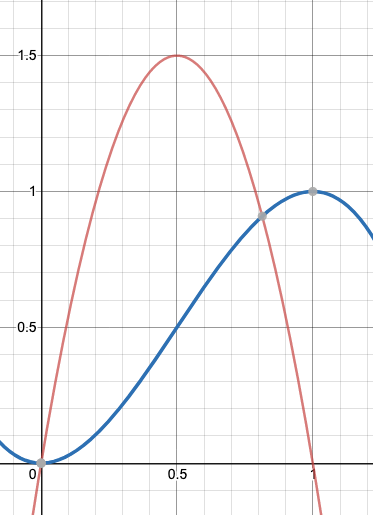
\includegraphics[width=6cm]{graph1}\\
    The red is $f(y)$ and the blue is $F(y)$. For values outside of the range, $[0,1]$, 
    the graph of $f(y)$ should be simply 0, and the graph of $F(y)$ should be 0 if $y < 0$ or 1 if $y > 1$.

\section*{Problem 4.134}
    
    \subsection*{(a)}
        In relation to the binomial distribution we have a probability $p = .7$, and $n = 10$,
        and we want the probability of at least $4$ successes. We get a probability of $1 - .011 = .989$.
    
    \subsection*{(b)}
            We do the same thing again, except this time we have $p = .6, n = 25$, and we want
            the probability of achieving at least 12 successes. This gives us $1 - .078 = .922$.

\section*{Problem 4.142}

    \subsection*{(a)}
        \begin{align*}
            m(t) &= E(e^{t Y})\\
            &= \int_0^1 e^{t y} f(y)dy\\
            &= \int_0^1 e^{t y} (1) dy\\
            &= \frac{1}{t} \int_0^t e^u du\\
            &= \frac{1}{t} [e^t - e^0]\\
            &= \frac{e^t - 1}{t}
        \end{align*}

    \subsection*{(b)}
        For the moment generating function for $W$.
        \begin{align*}
            m(t) &= E(e^{t W}) \\
            &= E(e^{t a Y})\\
            &= \int_0^1 e^{t a y} (1) dy \\
            &= \frac{1}{t a} \int_0^{t a} e^u du\\
            &= \frac{e^{ta} - 1}{ta}
        \end{align*}
        The distribution is still a uniform distribution because it is simply the same distribution except
        we are looking at the interval $(0, a)$.

    \subsection*{(c)}
        \begin{align*}
            m(t) &= E(e^{t X})\\
            &= E(e^{-t a Y})\\
            &= \int_0^1 e^{-t a y} dy\\
            &= \frac{1}{-ta} \int_0^{-ta} e^u du\\
            &= \frac{1}{ta} \int_{-ta}^0 e^u du\\
            &= \frac{1}{ta} [e^0 - e^{-ta}]\\
            &= \frac{1 - e^{-ta}}{ta}
        \end{align*}
        This will be a uniform distribution on the interval $(-a, 0)$.

    \subsection*{(d)}
        \begin{align*}
            m(t) &= E(e^{t V})\\
            &= E(e^{t(aY + b)})\\
            &= E(e^{t a Y}e^{t b})\\
            &= e^{t b} E(e^{t a Y})\\
            &= e^{t b} \frac{e^{ta} - 1}{ta}
        \end{align*}
        This will be a uniform distribution over the interval $(b, a+b)$ since the relationship between 
        $V$ and $Y$ transforms our unit interval to this interval.

\section*{Problem 4.190}
    
    \subsection*{(a)}
        Show that for an exponential density function, $r(t)$ is constant.
        \begin{proof}
            We wish to show that 
            \[
                r(t) = \frac{f(t)}{1- F(t)} = x, \ \ \ \forall t
            \]
            Let us first write out $f(t)$ and $F(t)$ explicitly,
            \[
                f(t) =
                \begin{cases}
                    \frac{1}{\beta}e^{-t / \beta}, & 0 \leq t < \infty\\
                    0, & \text{otherwise}
                \end{cases}
            \]
            Then if $y \leq 0, F(y) = 0$, and otherwise
            \begin{align*}
                F(t) &= \int_{-\infty}^t f(y) dy\\
                &= \int_0^t \frac{1}{\beta}e^{-y / \beta} dy\\
                &= \frac{1}{\beta} \int_0^t e^{-y / \beta} dy\\
                &= \frac{1}{\beta} \int_0^{- t / \beta} -\beta e^u du\\
                &= -\int_0^{- t / \beta} e^u du\\
                &= -[e^{- t / \beta} - e^0]\\
                &= -[e^{- t / \beta} - 1]\\
                &= 1 - e^{- t / \beta}
            \end{align*}
            So we say
            \[
                F(t) = 
                \begin{cases}
                    0 & t < 0\\
                    1 - e^{-t / \beta} & t \geq 0
                \end{cases}
            \]
            For any non-negative value of $t$, we have
            \begin{align*}
                r(t) &= \frac{\frac{1}{\beta}e^{-t / \beta}}{1- [1 - e^{-t / \beta}]}\\
                &= \frac{1}{\beta}\frac{e^{-t / \beta}}{e^{- t / \beta}}\\
                &= \frac{1}{\beta} e^{-t / \beta + t / \beta}\\
                & = \frac{1}{\beta}
            \end{align*}
            And we say that $r(t)$ is constant.
        \end{proof}

    \subsection*{(b)}
        Show that $r(t)$ is increasing.
        \begin{proof}
            First note that 
            \[
                f(y) = \frac{my^{m-1}}{\alpha}e^{-y^m / \alpha}, \ \ \ \ \ \ \ \ 0 \leq y < \infty, \alpha, m > 1
            \]
            Then we must compute $F(y)$.
            \begin{align*}
                F(y) &= \int_0^y f(t) dt\\
                &= \int_0^y \frac{mt^{m-1}}{\alpha}e^{-t^m / \alpha}dt \\
                &= \frac{m}{\alpha} \int_0^y t^{m - 1} e^{-t^m / \alpha} dt \\
                & = 1 - e^{-(y / \alpha)^m}\\
            \end{align*}
            Then we say that 
            \begin{align*}
                r(t) &= \frac{f(t)}{1- F(t)}\\
                &= \frac{\frac{mt^{m-1}}{\alpha}e^{-t^m / \alpha}}{1 - F(t)}\\
                &= \frac{\frac{mt^{m-1}}{\alpha}e^{-t^m / \alpha}}{1 - [1 - e^{-(t / \alpha)^m}]}\\
                &= \frac{\frac{mt^{m-1}}{\alpha}e^{-t^m / \alpha}}{e^{-(t / \alpha)^m}}\\
                &= \frac{mt^{m-1}}{\alpha} \cdot e^{(-t ^ m / \alpha) + (t / \alpha)^m}\\
                r'(t) &\geq 0 \ \ \forall m > 1 \Longrightarrow r(t) \text{ is increasing} 
            \end{align*}
        \end{proof}
\end{document}